The \verb+vga_drive+ module exists to handle the rendering of a 640x480 resolution image on the screen. 
The image that is supposed to be rendered consists of a background image previously 
stored in the SRAM consisting of pre filled bars that within the module will be blanked
out according to the input stimuli, which will give the appearance of bars being filled 
to different levels.   

To render an image on the vga screen you need five main signals. Three analog color channels (red, green and blue)
and two signals for synchronization hsync and vsync. The image is rendered pixel by pixel line by line using
a horizontal sweep pattern which is reset by the two sync signals. If a color is set when the sweep resets
arbitrary patterns can occur and therefore the signal has to be blanked during the reset phase.

The module \verb+vga_drive+ accomplishes this using eleven pipelined sub modules viewable in \ref{fig:vgadrive}
it has N inputs: volume\_input, balance\_inputs   

\begin{figure}[h]
        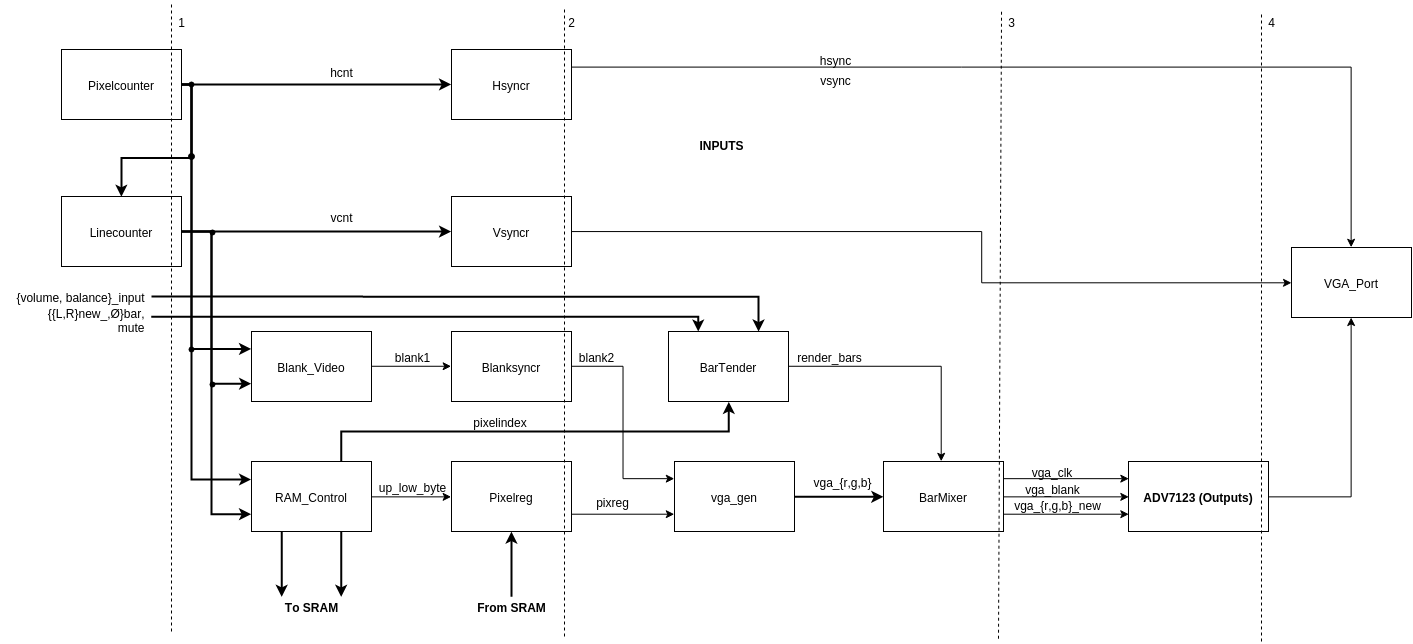
\includegraphics[scale=0.35]{vgadrive.png}
        \caption{Block diagram of vga\_drive}
        \label{fig:vgadrive}
\end{figure}



  \subsection{VGA\_driver:bartender}
  \subsection{VGA\_driver:barmixer}

